\documentclass[french,]{compterendu}
\usepackage{lmodern}
\usepackage{amssymb,amsmath}
\usepackage{ifxetex,ifluatex}
\usepackage{fixltx2e} % provides \textsubscript
\ifnum 0\ifxetex 1\fi\ifluatex 1\fi=0 % if pdftex
  \usepackage[T1]{fontenc}
  \usepackage[utf8]{inputenc}
\else % if luatex or xelatex
  \ifxetex
    \usepackage{mathspec}
  \else
    \usepackage{fontspec}
  \fi
  \defaultfontfeatures{Ligatures=TeX,Scale=MatchLowercase}
\fi
% use upquote if available, for straight quotes in verbatim environments
\IfFileExists{upquote.sty}{\usepackage{upquote}}{}
% use microtype if available
\IfFileExists{microtype.sty}{%
\usepackage{microtype}
\UseMicrotypeSet[protrusion]{basicmath} % disable protrusion for tt fonts
}{}
\usepackage[left=2cm,right=2cm,top=2cm,bottom=2.5cm]{geometry}
\usepackage{hyperref}
\hypersetup{unicode=true,
            pdftitle={Projet Analyse de données},
            pdfauthor={Léo GABET},
            pdfkeywords={Langage python maos zencore},
            pdfborder={0 0 0},
            breaklinks=true}
\urlstyle{same}  % don't use monospace font for urls
\ifnum 0\ifxetex 1\fi\ifluatex 1\fi=0 % if pdftex
  \usepackage[shorthands=off,main=french]{babel}
\else
  \usepackage{polyglossia}
  \setmainlanguage[]{}
\fi
% Adding environment CSLReferences for compatibility with pandoc >= 2.8
% BEGIN

\newlength{\cslhangindent}
\setlength{\cslhangindent}{1.5em}
\newlength{\csllabelwidth}
\setlength{\csllabelwidth}{3em}
\newenvironment{CSLReferences}[2] % #1 hanging-ident, #2 entry spacing
 {% don't indent paragraphs
  \setlength{\parindent}{0pt}
  % turn on hanging indent if param 1 is 1
  \ifodd #1 \everypar{\setlength{\hangindent}{\cslhangindent}}\ignorespaces\fi
  % set entry spacing
  \ifnum #2 > 0
  \setlength{\parskip}{#2\baselineskip}
  \fi
 }%
 {}
\usepackage{calc} % for \widthof, \maxof
\newcommand{\CSLBlock}[1]{#1\hfill\break}
\newcommand{\CSLLeftMargin}[1]{\parbox[t]{\maxof{\widthof{#1}}{\csllabelwidth}}{#1}}
\newcommand{\CSLRightInline}[1]{\parbox[t]{\linewidth}{#1}}
\newcommand{\CSLIndent}[1]{\hspace{\cslhangindent}#1}

% END
\usepackage{longtable,booktabs}
\IfFileExists{parskip.sty}{%
\usepackage{parskip}
}{% else
\setlength{\parindent}{0pt}
\setlength{\parskip}{6pt plus 2pt minus 1pt}
}
\setlength{\emergencystretch}{3em}  % prevent overfull lines
\providecommand{\tightlist}{%
  \setlength{\itemsep}{0pt}\setlength{\parskip}{0pt}}
\setcounter{secnumdepth}{5}
% Redefines (sub)paragraphs to behave more like sections
\ifx\paragraph\undefined\else
\let\oldparagraph\paragraph
\renewcommand{\paragraph}[1]{\oldparagraph{#1}\mbox{}}
\fi
\ifx\subparagraph\undefined\else
\let\oldsubparagraph\subparagraph
\renewcommand{\subparagraph}[1]{\oldsubparagraph{#1}\mbox{}}
\fi

%%% Use protect on footnotes to avoid problems with footnotes in titles
\let\rmarkdownfootnote\footnote%
\def\footnote{\protect\rmarkdownfootnote}



%Mise en page
%\usepackage[left=2cm,right=2cm,top=2cm,bottom=2.5cm]{geometry}
%\usepackage{lastpage} %Pour numérotaion des pages
\usepackage{eso-pic} %pour l'image de fond de la page de garde
\usepackage{enumitem} %Pour personnaliser les listes à puces
\usepackage{fancyhdr}
\usepackage{xcolor}
\usepackage[T1]{fontenc}
\usepackage{amsthm}
%\usepackage{thmtools}

\usepackage[figure,table]{totalcount} % Pour avoir les nombres de figures, tables et théoremes
\usepackage{totcount} % Pour compter le nombre de références

%Gestion des tableaux
\usepackage{multirow}
\usepackage{float}
\floatplacement{table}{H}
\floatplacement{figure}{ht!}

%Divers
\usepackage{ifthen} %Gestion des instructions conditionnelles


\widowpenalty=10000
\clubpenalty=10000

%%%%%%%%%%%%%%%%%%%%%%%%%%%
%% Defining new counters %%
%%%%%%%%%%%%%%%%%%%%%%%%%%%

%% Compteur des références
\newtotcounter{citenum} 
\def\oldcite{}
\let\oldcite=\bibcite
\def\bibcite{\stepcounter{citenum}\oldcite}

\regtotcounter{figure}
\regtotcounter{table}
\regtotcounter{theorem}


%%%%%%%%%%%%%%%%%%%%%%%%%%%%%%%%%%%%%%%%%%%%%%%
%% Configuration des messages de type badbox %%
%%%%%%%%%%%%%%%%%%%%%%%%%%%%%%%%%%%%%%%%%%%%%%%

\widowpenalty=10000
\clubpenalty=10000


%%%%%%%%%%%%%%%%%%%%%%%%%%%%
%% Theorem environemments %%
%%%%%%%%%%%%%%%%%%%%%%%%%%%%


\theoremstyle{urcastyle}
\newtheorem{theorem}{Théorème}
\newtheorem{lemma}{Lemme}
\newtheorem{corollary}{Corollaire}
\newtheorem{proposition}{Proposition}
\newtheorem{definition}{Définition}
\newtheorem{example}{Exemple}

\theoremstyle{remark}
%\newtheorem*{proof}{Démonstration}


%%%%%%%%%%%%%%%%%%%%%%%%%%%%%%%%%%%%%%%%%%%%
%% Désignation des variables de la classe %%
%%%%%%%%%%%%%%%%%%%%%%%%%%%%%%%%%%%%%%%%%%%%

% Processing title
  \newcommand{\titlehead}{Projet Analyse de données}
  \title{Projet Analyse de données}
    % Processing authors
  \newcounter{nbaut}
  \setcounter{nbaut}{9} % Nombre d'auteurs
  \author{Léo GABET}
      \date{01 janvier 2024}

 \resume{BLABLA}
 \keywords{Langage python maos zencore.}

 \coefficient{50 \%}


  \email{\href{mailto:leo.gabet@etudiant.univ-reims.fr}{\nolinkurl{leo.gabet@etudiant.univ-reims.fr}}}
%\email{\href{mailto:leo.gabet@etudiant.univ-reims.fr}{\nolinkurl{leo.gabet@etudiant.univ-reims.fr}}}
\logouniv{logo_URCA.pdf}
\logoufr{logoSEN.pdf}
\date{01 janvier 2024}
\diplome{M2 SEP}
\anac{2023-2024}
\module{SEP0931}
\enseig{Emmanuelle Gauthérat}
\evaluation{PROJET ADD}

%% Passage des compteurs à la classe pour maketitle.
\totfig{\total{figure}}
\tottab{\total{table}}
\totref{\total{citenum}}
\tottheo{\total{theorem}}

%%%%%%%%%%%%%%%%%%%
%% Mise en forme %%
%%%%%%%%%%%%%%%%%%%


%Formatage en-têtes et pieds de pages
\pagestyle{fancy}
\fancyhead[L]{\small \titlehead}
%\fancyhead[C]{\small \textcolor{urcabrown}{\titlehead}}
\fancyhead[R]{}
\fancyfoot[l]{\small \ifnum\value{nbaut}=1 {\theauthor} \else {Léo GABET \textit{}\fi}}
\fancyfoot[C]{\small \it \theeval \ \themodule \ -- \theanac}
\fancyfoot[R]{\small \thepage\ / \pageref{LastPage}}
% \renewcommand{\headrule}{\hbox to\headwidth{%
%     \color{urcabrown}\leaders\hrule height \headrulewidth\hfill}}
% \renewcommand{\footrule}{\hbox to\headwidth{%
%     \color{urcabrown}\leaders\hrule height \headrulewidth\hfill}}
\renewcommand{\headrulewidth}{0.5pt}
\renewcommand{\footrulewidth}{0.5pt}

\renewcommand{\headrulewidth}{0.5pt}
\renewcommand{\footrulewidth}{0.5pt}

\fancypagestyle{plain}{%
\fancyhf{} % clear all header and footer fields
\fancyfoot[C]{\small \thepage\ / \pageref{LastPage}} % except the center
\renewcommand{\headrulewidth}{0pt}
\renewcommand{\footrulewidth}{0pt}}

\AtEndDocument{\thispagestyle{plain}}
% Pandoc header


%%%%%%%%%%%%%%%%%%%%%%%
%% Début du document %%
%%%%%%%%%%%%%%%%%%%%%%%

\begin{document}

\AddToShipoutPictureBG*{
\includegraphics[width=\paperwidth,height=\paperheight]{fond_a4_sen_3.pdf}}

% \theoremstyle{urca}
\newtheorem{lemme}{Lemme}[section]
\newtheorem{theoreme}{Théorème}[section]
% \newtheorem{proposition}{Proposition}[section]
% \newtheorem{definition}{Définition}[section]
\newtheorem{corollaire}{Corollaire}[section]
\newtheorem{propriete}{Propriété}[section]
\newtheorem{proprietes}{Propriétés}[section]



\maketitle

% \pagebreak
% 
% % \begin{abstract}
% BLABLA
% \end{abstract}
% 

\vspace{1cm}

  {
  \hypersetup{linkcolor=black}
  \setcounter{tocdepth}{2}
  \pagebreak
  \tableofcontents
  }

\pagebreak
\normalsize



\hypertarget{introduction}{%
\section{Introduction}\label{introduction}}

\hypertarget{contexte-de-luxe9tude}{%
\subsection{Contexte de l'étude}\label{contexte-de-luxe9tude}}

Le vélo est devenu un mode de transport de plus en plus populaire à travers le monde, offrant une alternative écologique et saine aux moyens de déplacement traditionnels. En France, l'a promotion de 'intérêt de l'utilisation du vélo est devenue une priorité, avec des efforts déployés pour créer des infrastructures adaptées, telles que des pistes cyclables, afin de favoriser la sécurité des cyclistes et encourager la pratique du vélo.

Cependant, malgré ces initiatives, la sécurité des cyclistes sur les routes reste une préoccupation majeure. Les accidents de vélos peuvent avoir des conséquences graves, mettant en lumière la nécessité d'une compréhension approfondie des facteurs contribuant à ces incidents. Dans ce contexte, l'analyse de données offre une approche précieuse pour examiner les tendances, les corrélations et les déterminants des accidents de vélos en France.

Cette analyse s'appuiera sur deux jeux de données différents. D'une part, une base de données détaillant les accidents de vélos survenus à travers le pays fournira des informations précieuses sur les circonstances, la gravité et les lieux des incidents. D'autre part, une base de données spécifique à Paris, décrivant la création et l'emplacement des pistes cyclables, permettra d'explorer la corrélation entre l'infrastructure dédiée aux cyclistes et la fréquence des accidents.

L'objectif de cette analyse est de dégager des tendances significatives, de mettre en évidence les zones à risque élevé, et d'évaluer l'impact des pistes cyclables sur la sécurité des cyclistes. En comprenant les facteurs sous-jacents aux accidents de vélos, il devient possible d'orienter les politiques publiques, d'améliorer les infrastructures et de promouvoir des mesures préventives pour garantir une cohabitation sûre et efficace entre les cyclistes et les autres usagers de la route.

Cette étude contribuera ainsi à la promotion d'une mobilité durable, en mettant en lumière les défis actuels et en proposant des solutions basées sur des données probantes pour renforcer la sécurité des cyclistes en France.

\hypertarget{donnuxe9es}{%
\subsection{Données}\label{donnuxe9es}}

Les jeux de données comprennent une couverture complète des accidents de vélo à l'échelle nationale en France disponibles sur le site \textbf{data gouv}\footnote{\url{https://www.data.gouv.fr/fr/datasets/accidents-de-velo/\#/resources}}, offrant une vue d'ensemble des incidents survenus dans tout le pays. Un second jeu de données se concentre spécifiquement sur les pistes cyclables provenant du site \textbf{data Paris}\footnote{\url{https://opendata.paris.fr/explore/dataset/reseau-cyclable/information}}, cartographiant l'infrastructure dédiée dans diverses localités. Enfin, un troisième jeu de données se focalise sur les accidents de vélo à Paris (filtré de notre première base de donnée avec rajout des arrondissements). Ces ensembles de données permettent d'analyser les tendances, de localiser les zones à risques et d'évaluer l'impact des pistes cyclables sur la sécurité, offrant ainsi une compréhension approfondie de la situation des cyclistes en France.

\hypertarget{plan-de-luxe9tude}{%
\subsection{Plan de l'étude}\label{plan-de-luxe9tude}}

Notre première étape consistera à dégager les tendances des accidents de vélos et à localiser les zones à risques élevés à l'échelle nationale.

La deuxième phase de notre étude se concentrera sur l'analyse de la base de données détaillant les pistes cyclables à Paris. Cette démarche vise à cartographier ces infrastructures et à examiner leur évolution au fil du temps. Comprendre ces dynamiques est essentiel pour évaluer l'influence de l'infrastructure sur la sécurité des cyclistes.

Enfin, nous terminerons par regarder les données d'accidents par arrondissement de Paris permettant ainsi de cerner les défis spécifiques rencontrés dans la capitale. Cette approche nous permettra de déterminer les liens entre les accidents de vélos et l'existence de pistes cyclables. L'objectif ultime est d'identifier des zones spécifiques nécessitant des améliorations ciblées afin de renforcer la sécurité des cyclistes dans la ville de Paris.

\hypertarget{analyse}{%
\section{Analyse}\label{analyse}}

\hypertarget{les-accidents-de-vuxe9los-uxe0-luxe9chelle-nationale}{%
\subsection{Les accidents de vélos à l'échelle nationale}\label{les-accidents-de-vuxe9los-uxe0-luxe9chelle-nationale}}

Au-delà des chiffres et des statistiques, une exploration visuelle des données sur les accidents de vélos offre des perspectives riches et nuancées. Le graphique ci-dessous, fruit d'une lecture attentive des informations recueillies sur une période de 13 ans, se présente comme une fenêtre captivante sur les schémas temporels de ces incidents. En se plongeant dans les nuances des mois et des jours de la semaine, ce graphique met en évidence des tendances saisissantes, confirmant ainsi nos premières observations. Découvrons ensemble la corrélation entre les saisons, les moments de la journée et la fréquence des accidents, éléments clés pour une compréhension approfondie des dynamiques complexes entourant la sécurité des cyclistes sur nos routes.

\begin{figure}[H]

{\centering 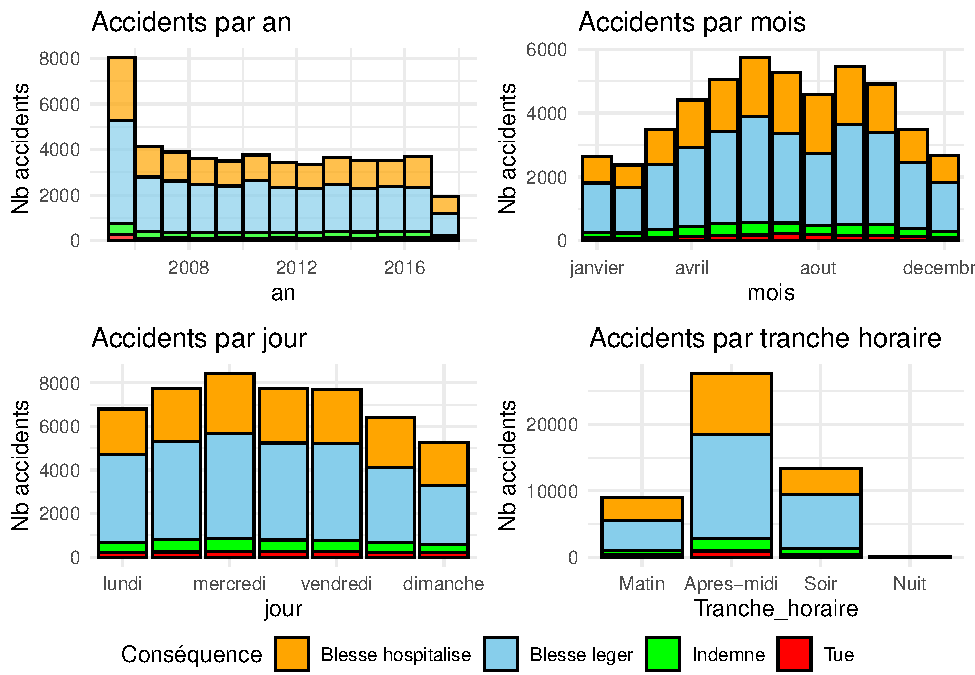
\includegraphics[width=0.9\linewidth]{Rapport_ADD_LEO-GABET_files/figure-latex/accfrancedetail-1} 

}

\caption{Représentation des accidents de vélo en France par année, mois, jour et horaire}\label{fig:accfrancedetail}
\end{figure}

\emph{\textbf{Lecture graphique} : Les accidents de vélos se déroulent principalement durant les mois à température douce voir chaude, tel que le mois de juin qui représente un pic des accidents de vélos sur 13 ans. On contaste bien que le type de jour lié aux accidents correspond aux jours de la semaine, avec une très grande part d'accident lors des après-midi.}

Au regard des données, plusieurs hypothèses émergent pour expliquer les schémas observés dans les accidents de vélo. L'augmentation des incidents pendant les mois chauds suggère une affluence plus importante de cyclistes par temps agréable. La concentration d'accidents en juin pourrait résulter de la fin de l'année scolaire, incitant potentiellement les jeunes à être plus actifs à vélo. Les après-midis se distinguent par une fréquence élevée d'incidents, probablement liée à la routine quotidienne et aux déplacements après le travail ou l'école. Les conditions de visibilité réduite en après-midi pourraient également contribuer à l'augmentation des accidents. De plus, les variations saisonnières et les moments de la journée semblent influencer les comportements des cyclistes, impactant ainsi le nombre d'accidents. Ces hypothèses fournissent une première approche pour interpréter les tendances, mais des analyses plus approfondies sont nécessaires pour confirmer ces impressions préliminaires.

\hypertarget{identification-des-zones-uxe0-risques-uxe9levuxe9s-uxe0-luxe9chelle-du-pays}{%
\subsubsection{Identification des zones à risques élevés à l'échelle du pays}\label{identification-des-zones-uxe0-risques-uxe9levuxe9s-uxe0-luxe9chelle-du-pays}}

\begin{figure}[H]

{\centering 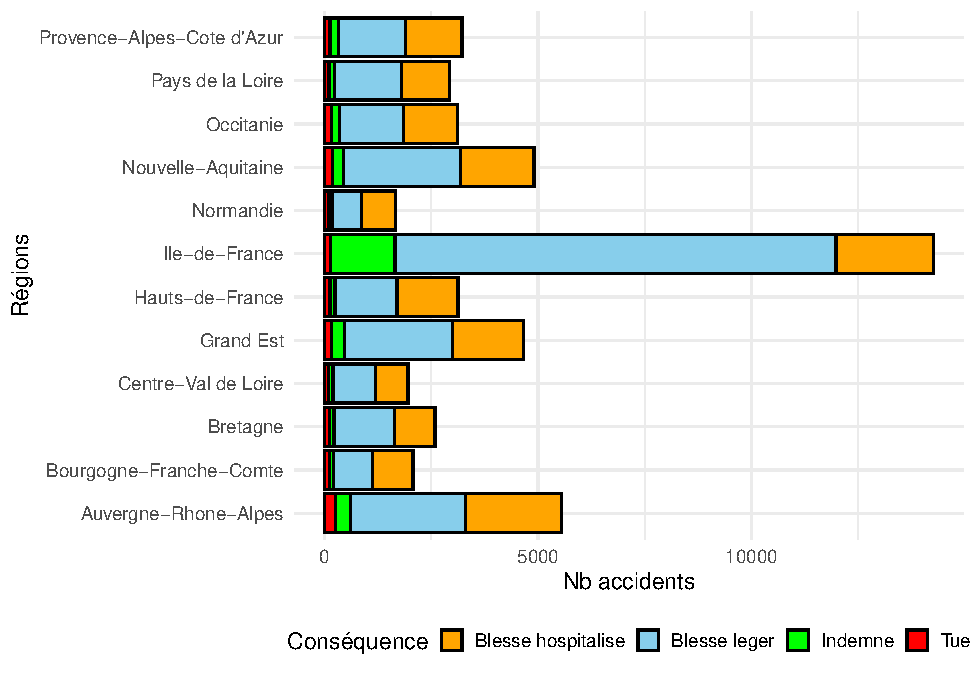
\includegraphics[width=0.9\linewidth]{Rapport_ADD_LEO-GABET_files/figure-latex/accfranceregion-1} 

}

\caption{Accidents en France en fonction des régions}\label{fig:accfranceregion}
\end{figure}

\emph{\textbf{Lecture graphique} : Une grande partie des accidents de vélo en France se déroule principalement en île de France, avec une très faible présence d'accidence en Provence-Alpes-Cote d'Azur (et Corse).}

La carte des accidents de vélo met en lumière une disparité significative entre les régions françaises. L'Île-de-France, avec sa densité de population et son réseau routier complexe, émerge comme une zone à risque élevé, reflétant peut-être l'intensité des déplacements urbains à vélo. En revanche, la faible incidence en Provence-Alpes-Côte d'Azur et en Corse soulève des questions intrigantes sur les facteurs qui contribuent à ce phénomène. Les différences dans l'infrastructure cyclable, les habitudes de déplacement, ou même les conditions météorologiques pourraient jouer un rôle clé dans cette disparité régionale.

\hypertarget{facteurs-et-contextes}{%
\subsubsection{Facteurs et contextes}\label{facteurs-et-contextes}}

\begin{figure}[H]

{\centering 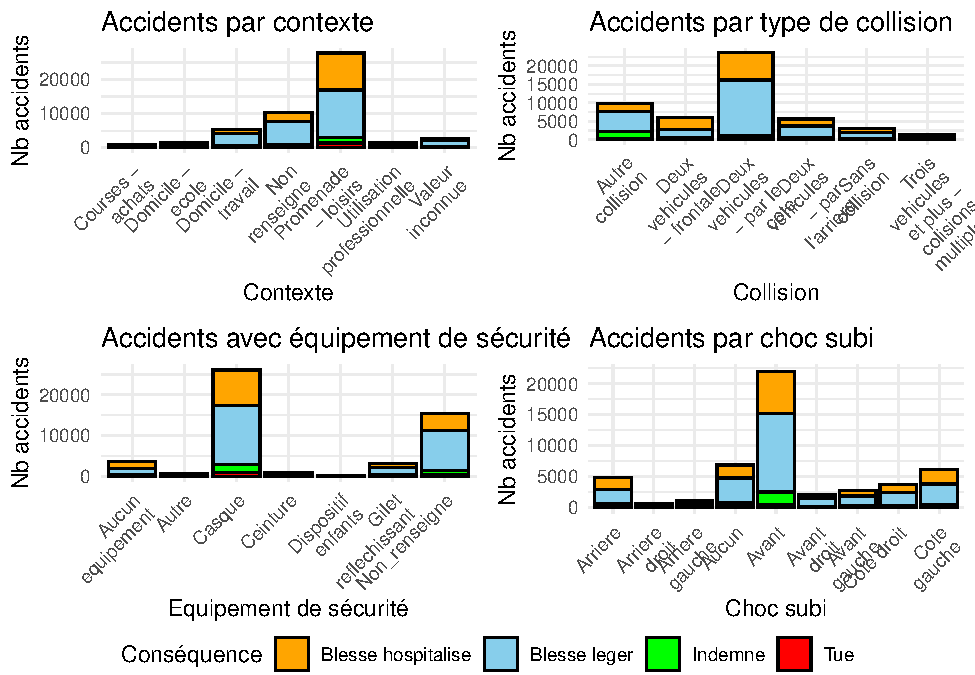
\includegraphics[width=0.9\linewidth]{Rapport_ADD_LEO-GABET_files/figure-latex/accCONTEXTE-1} 

}

\caption{Représentation des accidents de vélo en France par les contextes des collisions et choc subi avec les équipements de sécurités}\label{fig:accCONTEXTE}
\end{figure}

\emph{\textbf{Lecture graphique} : C'est lors de promenade et loisirs que les accidents de vélos se produisent le plus souvent, notamment par les voitures sur les cotés provoquant pour la plus part des chocs avant. On relève néanmoins que la plus part des accidentés possèdent au minima un casque pour leur équipement de sécurité, ce qui pourrait expliqué la forte présence de la conséquence ``blessé léger''.}

Les données dévoilent un panorama où les escapades récréatives et les moments de détente sont les principaux catalyseurs des accidents de vélo reflètent bien l'utilisation du vélo au quotidient.
Les rencontres avec des voitures sur les côtés, souvent associées à des chocs frontaux, émergent comme des scénarios prédominants. Cette tendance soulève des questions sur les interactions spécifiques entre les cyclistes et les véhicules, ainsi que sur les conditions routières pendant ces moments particuliers. En effet, ces accidents sont causés par beaucoup de conducteurs inattentif au volant, mais aussi certainement par des cyclistes qui ne respectent pas toujours le code de la route.
Malgrès tout, l'observation selon laquelle la majorité des accidentés portent au moins un casque constitue un point intéressant. Cette précaution pourrait expliquer en partie la fréquence élevée des conséquences répertoriées comme ``blessé léger'', mais aussi de l'effet important de la prévoyance de porter un casque de sécurité lorsqu'on fait du vélo.

\hypertarget{infrastructures-cyclables-uxe0-paris}{%
\subsection{Infrastructures Cyclables à Paris}\label{infrastructures-cyclables-uxe0-paris}}

\hypertarget{amuxe9nagement-des-pistes-cyclables-au-fil-du-temps}{%
\subsubsection{Aménagement des pistes cyclables au fil du temps}\label{amuxe9nagement-des-pistes-cyclables-au-fil-du-temps}}

\begin{figure}[H]

{\centering 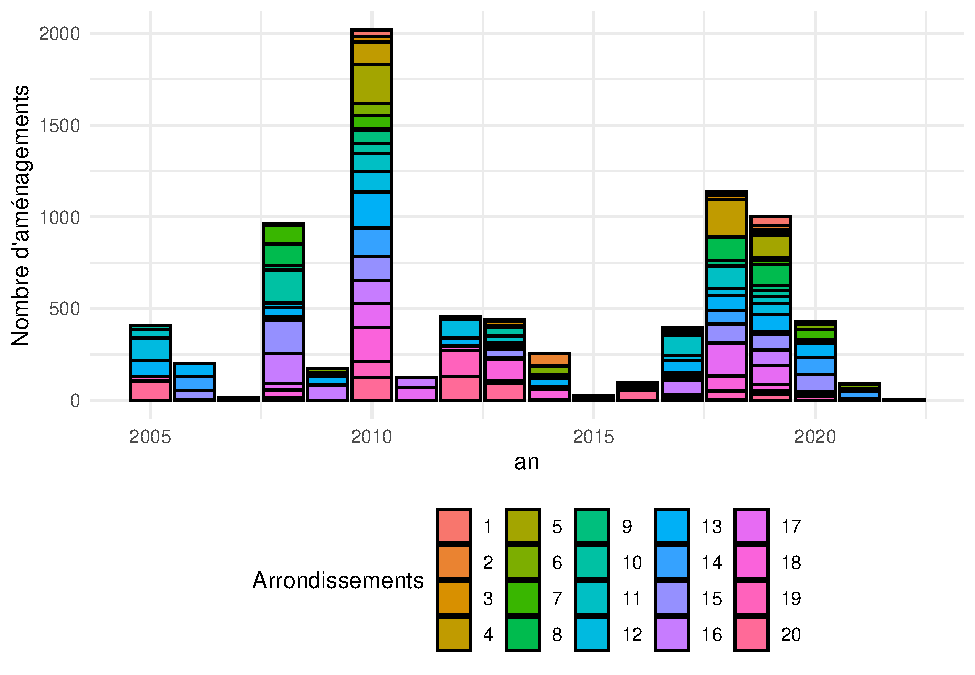
\includegraphics[width=0.9\linewidth]{Rapport_ADD_LEO-GABET_files/figure-latex/arrPARISdetails-1} 

}

\caption{Évolution des pistes cyclables dans les arrondissements au fil des années}\label{fig:arrPARISdetails}
\end{figure}

\emph{\textbf{Lecture graphique} : On remarqu'en 2010, beaucoup d'aménagement ont été effecuté dans l'ensemble des arrondissements de Paris. Cependant, on constate que le deuxième arrondissement possède le moins d'aménagement de piste cyclable ! De plus, pas mal de travaux d'aménagement ont lieu entre 2016 et 2019, ce qui pourrai expliqué la présence d'un pic d'accident de vélo dans Paris étant donné que les cyclistes n'avaient donc pas de pistes cyclables de présent pour rouler dessus.}

L'effort consacré aux aménagements cyclables à Paris en 2010 témoigne d'une volonté de favoriser la mobilité douce. Toutefois, la disparité dans la distribution de ces aménagements, en particulier dans le deuxième arrondissement, suscite des questions sur les priorités d'urbanisme et les défis potentiels pour les cyclistes dans cette zone spécifique.
La période de travaux intensive entre 2016 et 2019 offre un contexte temporel intrigant, suggérant que l'absence de pistes cyclables opérationnelles pourrait avoir contribué à un pic d'accidents de vélo dans Paris. Les cyclistes, privés d'infrastructures dédiées, pourraient avoir été confrontés à des conditions moins sécurisées, soulignant l'importance cruciale de l'infrastructure cyclable dans la prévention des accidents.

\hypertarget{type-damuxe9nagement}{%
\subsubsection{Type d'aménagement}\label{type-damuxe9nagement}}

\begin{figure}[H]

{\centering 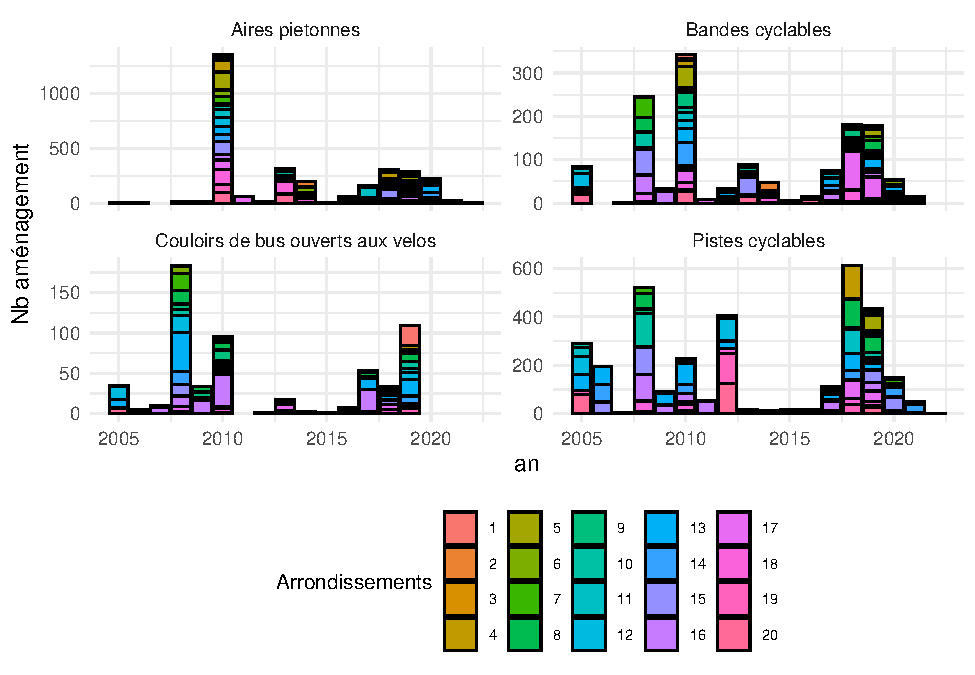
\includegraphics[width=0.9\linewidth]{Rapport_ADD_LEO-GABET_files/figure-latex/arrPARISTypo-1} 

}

\caption{Évolution des typologies selon les arrondissements au fil des années}\label{fig:arrPARISTypo}
\end{figure}

\emph{\textbf{Lecture graphique} : On voit donc que selon les différentes typologies d'aménagements où les vélos peuvent circulés, les pistes et bandes cyclables dominent, avec encore une fois par exemple le faite que le deuxième arrondissement possède le moins d'aménagement pour les vélos.}

L'écrasante prédominance des pistes et bandes cyclables dans le paysage des aménagements pour les vélos suggère une attention particulière portée à ces infrastructures. Cependant, la constatation que le deuxième arrondissement est à la traîne en matière d'aménagements souligne l'importance de la planification urbaine ciblée pour garantir une accessibilité équitable et sécurisée pour tous les cyclistes. Il ne faut pas oublier aussi que le duexième arrondissement n'est autre que le centre de Paris, donc un lieu très visité avec une circulation intensive de vélos, passants et voitures.
Cette disparité pourrait influencer directement l'expérience des cyclistes dans le deuxième arrondissement, les exposant potentiellement à des conditions de circulation moins optimales.
En synthèse, l'analyse des différents types d'aménagements souligne l'importance de la qualité et de la répartition équitable des infrastructures pour assurer une expérience cycliste sûre et agréable à travers Paris.

\hypertarget{les-accidents-de-vuxe9los-uxe0-paris}{%
\subsection{Les accidents de vélos à Paris}\label{les-accidents-de-vuxe9los-uxe0-paris}}

Nous allons nous concentré sur les années 2016, 2017 et 2018 qui représentent un très grand nombre d'accident pour Paris.

\begin{figure}[H]

{\centering 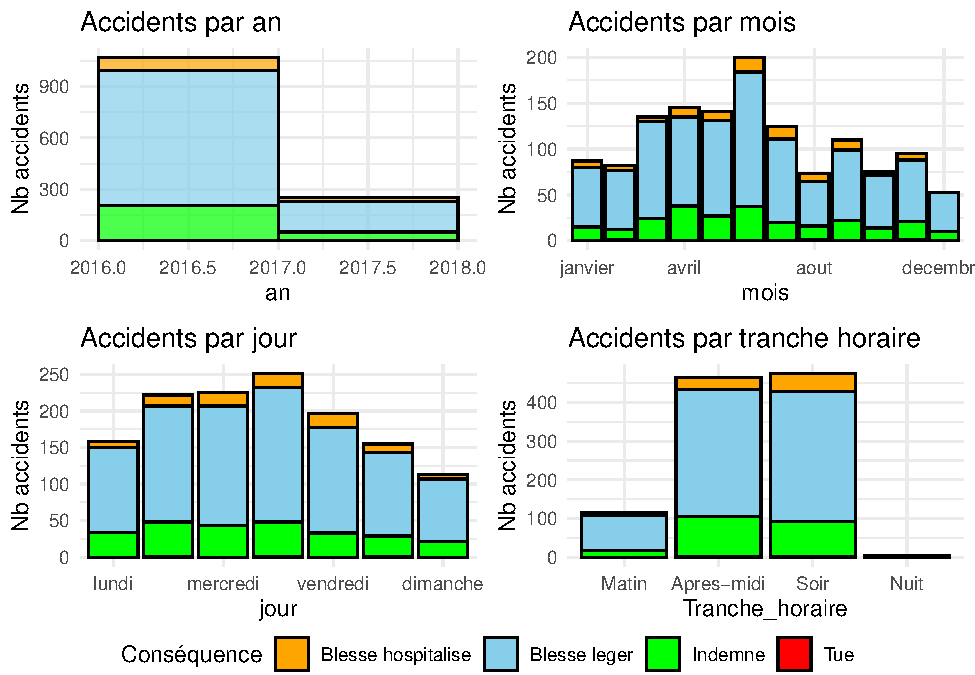
\includegraphics[width=0.9\linewidth]{Rapport_ADD_LEO-GABET_files/figure-latex/accParisdetail-1} 

}

\caption{Représentation des accidents de vélo à Paris par année, mois, jour et horaire}\label{fig:accParisdetail}
\end{figure}

\emph{\textbf{Lecture graphique} : Nous retrouvons une analyse similaire à l'echelle de la France entière avec cependant un plus grand nombre d'acccident lors du soir.}

La métropole, particulièrement propice aux déplacements à vélo, voit une augmentation des incidents pendant les mois chauds, ce qui pourrait être attribuable à la forte présence de cyclistes profitant des conditions estivales. Le pic en juin pourrait également être amplifié par la fin de l'année scolaire, incitant les jeunes parisiens à être plus actifs à vélo.
Concernant les après-midis, la routine quotidienne parisienne, marquée par les déplacements fréquents après le travail ou l'école, pourrait expliquer la concentration d'accidents pendant cette période. Les conditions de visibilité réduite en après-midi, peut-être accentuées par l'ombre des bâtiments emblématiques de Paris, pourraient jouer un rôle dans cette tendance.
Les variations saisonnières et les particularités de la routine quotidienne parisienne influencent ainsi les comportements des cyclistes, impactant le nombre d'accidents.

\hypertarget{identification-des-arrondissements-uxe0-risques-uxe9levuxe9s}{%
\subsubsection{Identification des arrondissements à risques élevés}\label{identification-des-arrondissements-uxe0-risques-uxe9levuxe9s}}

\begin{figure}[H]

{\centering 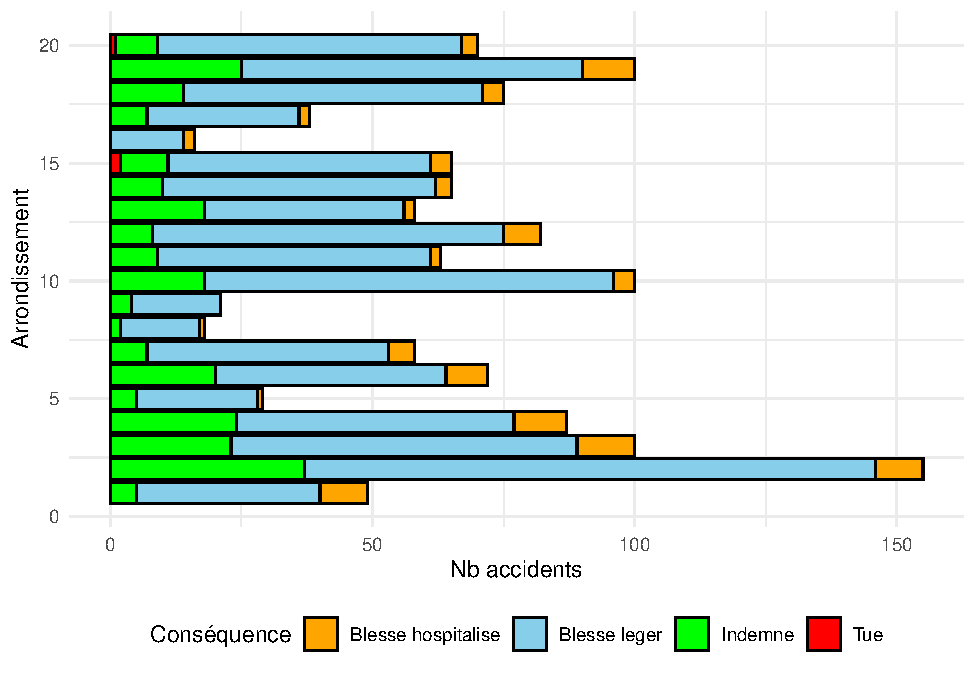
\includegraphics[width=0.9\linewidth]{Rapport_ADD_LEO-GABET_files/figure-latex/arrPARISaccident-1} 

}

\caption{Les accidents de vélos selon les arrondissements de Paris}\label{fig:arrPARISaccident}
\end{figure}

\emph{\textbf{Lecture graphique} : Sans surprise, le 2ème arrondissement possède la majorité des accidents de vélos suivi des 3ième, 10ième, 19ième et 20ième arrondissements. Concernant le 2ième arrondissement, une simple hypothèse viendrait du faite qu'il s'agit du centre même de Paris, donc la localisation qui regroupe le plus de personnes ! et d'autre part, nous avons aussi vu que le nombre d'aménagement étaient très bas dans cet arrondissement.}

Le 2ème arrondissement, étant le centre névralgique de Paris, se caractérise par une activité frénétique et une densité de population élevée. Cette situation peut contribuer à une fréquence plus élevée d'accidents de vélo, en raison du volume important de déplacements dans cette zone centrale. De plus, comme précédemment observé, le faible nombre d'aménagements cyclables dans le 2ème arrondissement pourrait accentuer les risques d'incidents.
Quant aux autres arrondissements cités, des analyses plus approfondies pourraient explorer des facteurs spécifiques tels que la topographie, la densité de circulation, ou la présence d'aménagements dédiés dans ces zones.
Cette observation renforce l'idée que la sécurité des cyclistes à Paris dépend fortement de la combinaison entre la densité de population, les caractéristiques géographiques et la disponibilité d'infrastructures adaptées. Des mesures ciblées, notamment dans les zones centrales à forte fréquentation, pourraient être cruciales pour réduire le nombre d'accidents de vélo dans la capitale.

\hypertarget{facteurs-et-contextes-1}{%
\subsubsection{Facteurs et contextes}\label{facteurs-et-contextes-1}}

\begin{figure}[H]

{\centering 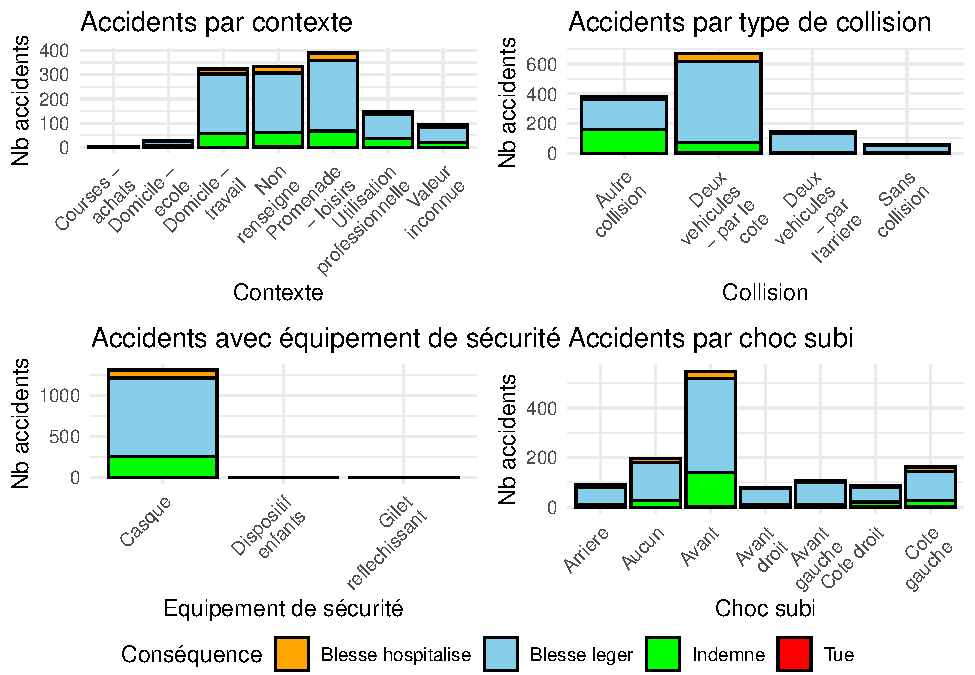
\includegraphics[width=0.9\linewidth]{Rapport_ADD_LEO-GABET_files/figure-latex/accCONTEXTE2-1} 

}

\caption{Représentation des accidents de vélo à Pairs par les contextes des collisions et choc subi avec les équipements de sécurités}\label{fig:accCONTEXTE2}
\end{figure}

\emph{\textbf{Lecture graphique} : Tout comme à l'echelle de la France entière, nous retrouvons des similitudes, cependant on constate que c'est aussi lors des trajets pour aller au travail que les accidents se produisent et lors d'utilisation professionelle en plus des promenades de loisirs. Il y a aussi une majorité d'accident de type blessé léger, ce qui rejoint le fait que la quasi totalité possèdent un casque de sécurité.}

À Paris, les trajets domicile-travail sont des moments sensibles, probablement influencés par la densité de la circulation et les défis liés à la navigation urbaine. L'utilisation professionnelle des vélos, peut-être liée aux livraisons ou aux déplacements professionnels, contribue également aux incidents. Ces observations soulignent la nécessité de politiques de sécurité routière spécifiquement adaptées aux besoins des cyclistes urbains parisiens.
La prédominance d'accidents classés en ``blessé léger'' s'explique en partie par la généralisation du port de casques de sécurité. Ceci suggère que bien que les accidents surviennent, les dispositifs de sécurité individuels peuvent atténuer la gravité des blessures. Cependant, il demeure crucial d'investir dans la prévention pour réduire le nombre d'accidents à la source.
En somme, cette analyse locale renforce l'idée que les particularités de Paris en matière de déplacements urbains influent sur les tendances des accidents de vélo, soulignant l'importance de mesures de sécurité routière adaptées à la dynamique spécifique de la capitale.

\hypertarget{conclusions-et-perspectives}{%
\section{Conclusions et perspectives}\label{conclusions-et-perspectives}}

L'exploration approfondie des données sur les accidents de vélos offre un aperçu significatif des tendances et des défis associés à la sécurité des cyclistes. Durant la période de 2016 à 2018, une augmentation notable des incidents a été constatée, suscitant l'intérêt pour des recherches complémentaires visant à identifier les facteurs socio-économiques et environnementaux qui ont pu contribuer à cette hausse.

Le mois de juin se révèle être une période critique, soulignant la nécessité de campagnes de sensibilisation saisonnières pour renforcer les comportements sécuritaires des cyclistes. L'analyse des jours de la semaine et des tranches horaires met en lumière des moments spécifiques où des mesures de prévention renforcées pourraient être mises en œuvre pour réduire les risques.

La concentration d'accidents en Île-de-France met en exergue l'importance d'investissements ciblés dans l'infrastructure cyclable de cette région. Des améliorations significatives pourraient être apportées en tenant compte des données sur les zones à risque élevé.

Les accidents liés aux activités de loisir soulignent l'importance de sensibiliser les cyclistes non seulement en tant qu'utilisateurs de transport, mais aussi en tant que participants à des loisirs. Des campagnes éducatives spécifiques pourraient encourager des comportements prudents dans ces contextes particuliers.

L'analyse détaillée de Paris entre 2016 et 2018 révèle des disparités significatives entre les arrondissements, avec le 2ème arrondissement enregistrant le plus grand nombre d'accidents. Ce constat met en évidence la nécessité d'une planification urbaine plus attentive et d'un renforcement des aménagements cyclables, en particulier dans les zones à risque élevé.

En se penchant sur les types de collisions et l'équipement de sécurité, la tendance de comportements responsables et de l'utilisation d'équipements de protection peut jouer un rôle clé dans la réduction des blessures graves. La moyenne d'âge des victimes suggère également la nécessité d'adapter les programmes de sécurité routière pour atteindre un public diversifié, des jeunes adultes aux personnes plus âgées.

En conclusion, cette analyse offre des perspectives pour orienter les efforts de prévention et d'aménagement urbain, soulignant l'importance de l'engagement communautaire, de la sensibilisation continue et de la collaboration entre les autorités locales et les parties prenantes pour créer des environnements plus sûrs pour les cyclistes.

\hypertarget{annexes}{%
\section{Annexes}\label{annexes}}

\hypertarget{base-de-donnuxe9es}{%
\subsection{Base de données}\label{base-de-donnuxe9es}}

Mettre ici les natures des variables

\hypertarget{compluxe9ment}{%
\subsection{Complément}\label{compluxe9ment}}

\begin{figure}[H]

{\centering 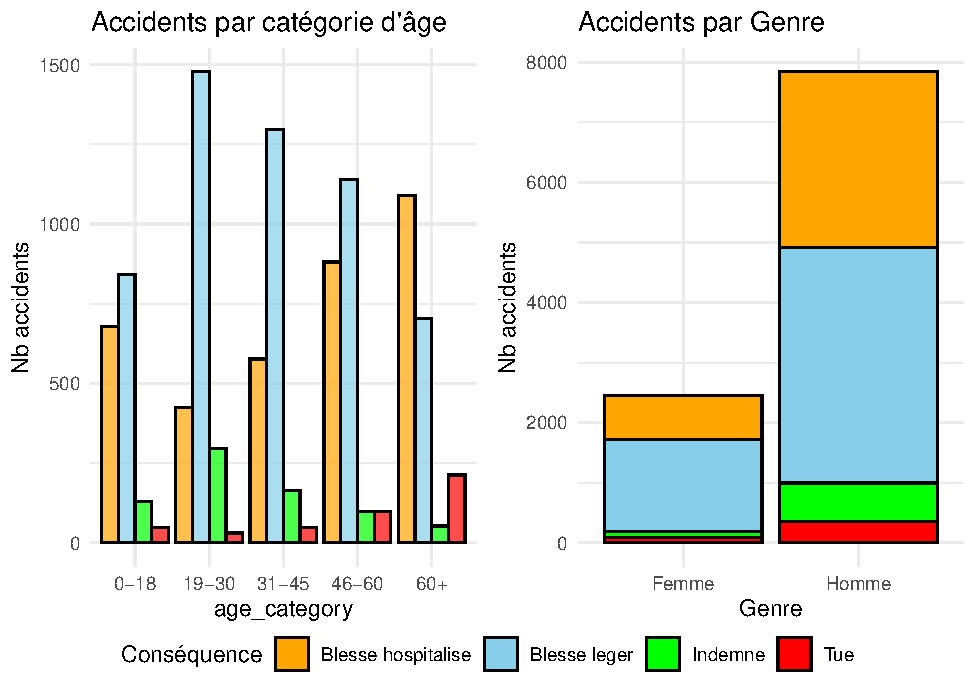
\includegraphics[width=0.9\linewidth]{Rapport_ADD_LEO-GABET_files/figure-latex/accfranceComple-1} 

}

\caption{Représentation des accidents de vélo en France par catégorie d'âge et genre}\label{fig:accfranceComple}
\end{figure}

\hypertarget{acp-sur-nos-variables-quantitatives-annuxe9e-uxe2ge-et-duxe9partement}{%
\subsection{ACP sur nos variables quantitatives année, âge et département}\label{acp-sur-nos-variables-quantitatives-annuxe9e-uxe2ge-et-duxe9partement}}

Voici une interprétation plus spécifique en considérant les variables ``an'' (année), ``dep'' (département), et ``age'' (âge) :

\begin{verbatim}
## 
## Call:
## PCA(X = data_quantitative, scale.unit = TRUE, graph = FALSE) 
## 
## 
## Eigenvalues
##                        Dim.1   Dim.2   Dim.3
## Variance               1.219   0.987   0.794
## % of var.             40.644  32.890  26.465
## Cumulative % of var.  40.644  73.535 100.000
## 
## Individuals (the 10 first)
##         Dist    Dim.1    ctr   cos2    Dim.2    ctr   cos2    Dim.3    ctr
## 1   |  3.420 | -2.138  0.037  0.391 | -2.631  0.068  0.592 |  0.451  0.002
## 2   |  3.018 | -2.030  0.033  0.452 | -0.445  0.002  0.022 |  2.189  0.059
## 3   |  3.261 | -2.418  0.047  0.550 |  0.065  0.000  0.000 |  2.187  0.059
## 4   |  2.921 | -2.078  0.035  0.506 | -0.759  0.006  0.068 |  1.906  0.045
## 5   |  2.971 | -2.150  0.037  0.524 | -0.586  0.003  0.039 |  1.965  0.047
## 6   |  3.033 | -1.583  0.020  0.272 | -0.596  0.004  0.039 |  2.517  0.078
## 7   |  2.953 | -1.440  0.017  0.238 | -0.943  0.009  0.102 |  2.399  0.071
## 8   |  2.909 | -2.211  0.039  0.578 | -1.301  0.017  0.200 |  1.371  0.023
## 9   |  2.937 | -1.194  0.011  0.165 | -1.684  0.028  0.329 |  2.088  0.054
## 10  |  3.073 | -1.360  0.015  0.196 | -2.362  0.055  0.591 |  1.419  0.025
##       cos2  
## 1    0.017 |
## 2    0.526 |
## 3    0.450 |
## 4    0.426 |
## 5    0.438 |
## 6    0.689 |
## 7    0.660 |
## 8    0.222 |
## 9    0.506 |
## 10   0.213 |
## 
## Variables
##        Dim.1    ctr   cos2    Dim.2    ctr   cos2    Dim.3    ctr   cos2  
## an  |  0.685 38.463  0.469 |  0.466 22.013  0.217 | -0.560 39.524  0.314 |
## age | -0.401 13.179  0.161 |  0.876 77.810  0.768 |  0.267  9.010  0.072 |
## dep |  0.768 48.357  0.590 |  0.042  0.177  0.002 |  0.639 51.466  0.409 |
\end{verbatim}

\begin{figure}[H]

{\centering 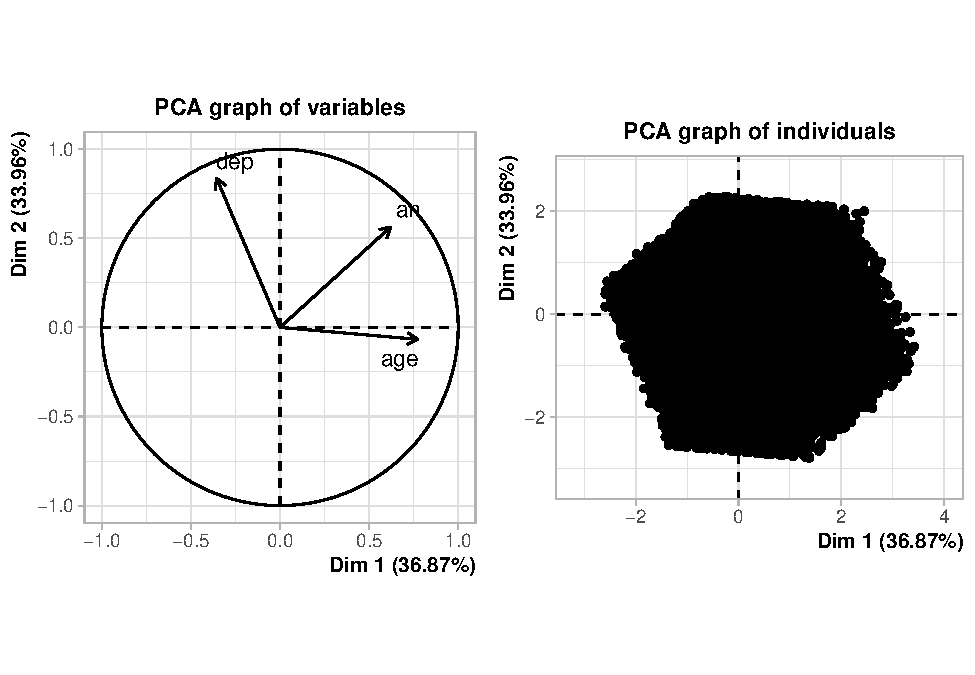
\includegraphics[width=0.9\linewidth]{Rapport_ADD_LEO-GABET_files/figure-latex/acp-1} 

}

\caption{ACP}\label{fig:acp}
\end{figure}

Les individus formant un cercle peuvent indiquer que les années, départements, et groupes d'âge sont liés d'une manière particulière. Cela pourrait signifier qu'il y a des années ou des départements où les accidents de vélo sont plus fréquents, ou que certaines tranches d'âge sont plus touchées. Comme nous l'avons vu, les départements de l'Ile de France, Nouvelle Aquitaine et Auvergne Rhone Alpes représentent une grande part de nos accidents dans notre base. De plus, nous avions vu un très grand nombre d'accident à partir de 2016 et une moyenne d'âge autour des 20/30 ans, ce qui est bien montré par notre ACP.

Ces résultats suggèrent que les années et les départements expliquent une grande partie de la variance, tandis que l'âge joue un rôle distinct.

Les valeurs élevées de \(cos^2\) indiquent une bonne représentation des années, départements et tranches d'âge dans l'espace des composantes principales. Par exemple, nous avons un \(cos^2\) de \(0.590\) pour la variable ``département'' sur le première axe et un \(cos^2\) de \(0.768\) pour la variable ``âge'' sur le deuxième axe.

Interprétation Globale :

\begin{itemize}
\tightlist
\item
  Les accidents de vélo sont influencés de manière significative par les années, les départements et les tranches d'âge.
\item
  La première composante principale peut représenter des variations temporelles et spatiales, la deuxième composante principale semble être liée à des différences liées à l'âge des personnes impliquées, et la troisième composante principale peut être une combinaison temporelle et spatiale.
\end{itemize}

\hypertarget{analyse-multivariuxe9}{%
\subsection{Analyse multivarié}\label{analyse-multivariuxe9}}

\hypertarget{acm-sur-les-accidents-de-vuxe9lo-en-france}{%
\subsubsection{ACM sur les accidents de vélo en France}\label{acm-sur-les-accidents-de-vuxe9lo-en-france}}

\begin{figure}[H]

{\centering 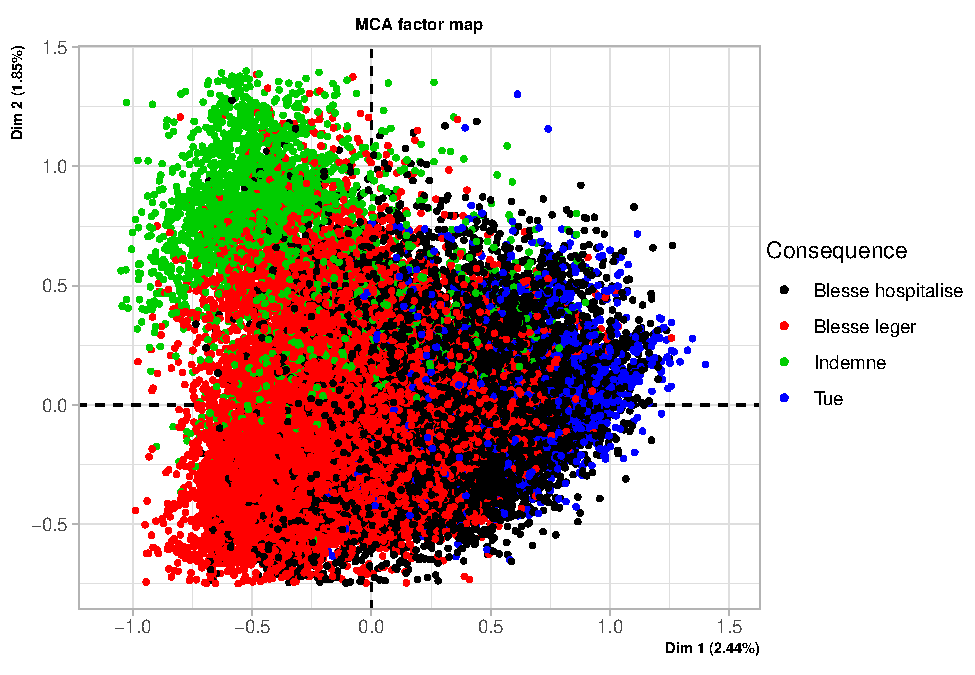
\includegraphics[width=0.9\linewidth]{Rapport_ADD_LEO-GABET_files/figure-latex/acm1-1} 

}

\caption{ACM1}\label{fig:acm1}
\end{figure}

Du graphe de l'ACM ressort 4 zones, dont :

\begin{itemize}
\tightlist
\item
  La zone indemne en vert en haut à gauche, associés aux modalités Tranche\_horaire\_nuit, Situation\_sur\_trottoir, nuit sans eclairage public, Choc subi aucun etc.
\item
  La zone Blessé léger en rouge qui représente la plus grosse partie de nos individu comme déjà vu ultérieurement, associé aux modalités Ile de France, Surface mouillé, Meteo pluie légère.
\item
  Les zones Blessé hospitalisé/Tué respectivement en noir/bleu qui se chevauche entre la partie rouge (blessé léger) et bleu (Tué) coté centré/droit de notre graphe, associés aux modalités Hors agglomération, Lieu Zone piétonne, Choc subi coté droit etc.
\end{itemize}

\begin{figure}[H]

{\centering 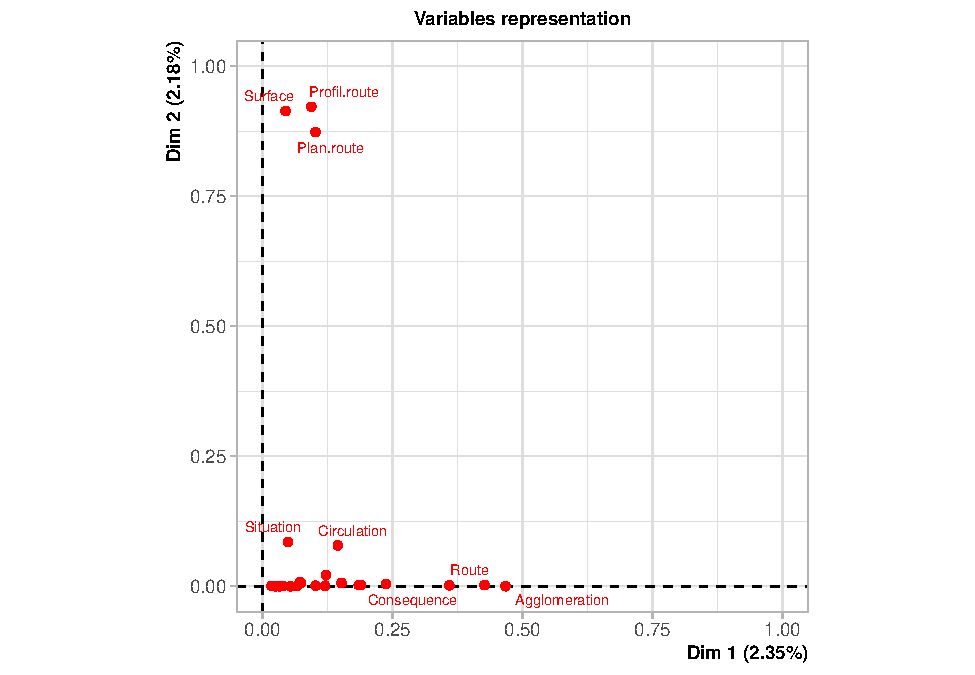
\includegraphics[width=0.9\linewidth]{Rapport_ADD_LEO-GABET_files/figure-latex/acm1moda-1} 

}

\caption{Modalité}\label{fig:acm1moda}
\end{figure}

On distingue que sur le premier axe, 4 variables se distinguent qui sont les conséquences, régions, routes et agglomérations. De plus, un autre groupe de 3 variables se distinguent sur le deuxième axe à savoir les surfaces, profils de routes et plans de routes.
Nous ne nous intéresserons qu'au premier axe, les modalités du deuxième axe sont très éloignés de notre groupe d'individu.

En regardant l'ACM en laissant seulement nos 4 variables avec leurs modalités, nous avons le graphe ci-dessous :

\begin{figure}[H]

{\centering 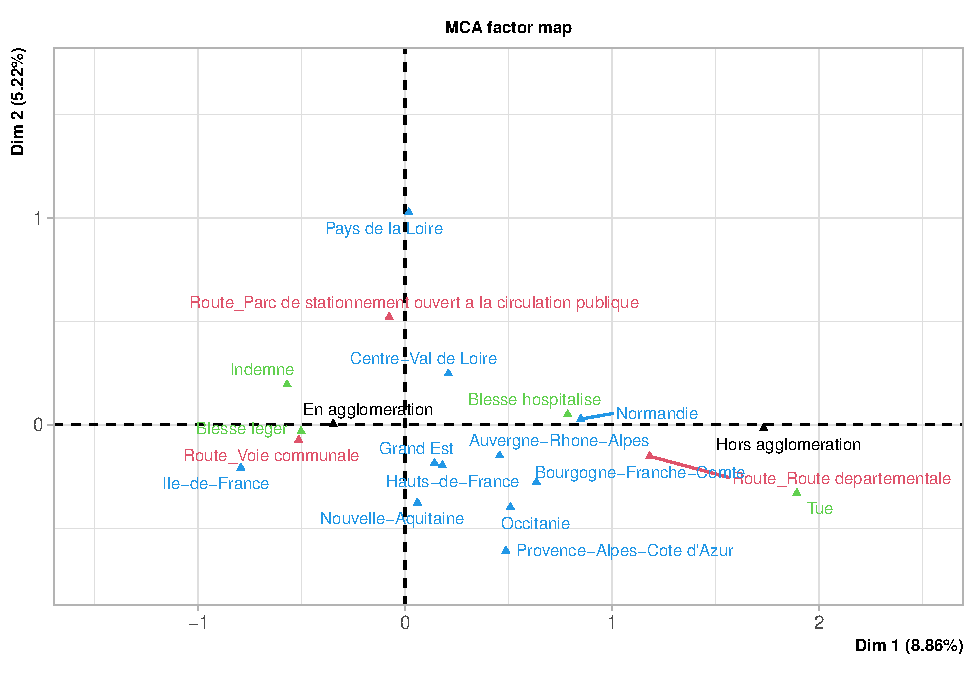
\includegraphics[width=0.9\linewidth]{Rapport_ADD_LEO-GABET_files/figure-latex/acm1modagraphe-1} 

}

\caption{Mises en évidences des modalités}\label{fig:acm1modagraphe}
\end{figure}

Ceci nous permet d'affiner notre analyse du début. En effet, on constate bien une séparation de notre graphe en deux parties. Une partie gauche reflétant les cas des accidents avec Indemne et Blessé léger qui se situe en agglomeration donc par exemple en Ile de France ! Puis une partie droite symbolisant les accidents plus grave se situant en hors agglomération comme en Auvergne-Rhone-Alpes.

Pour rappel, la variable contexte n'était pas si loin du groupe de nos 4 variables de notre premier axe, il serait donc intéressant d'analyser les variables régions, contexte et conséquence.

\begin{figure}[H]

{\centering 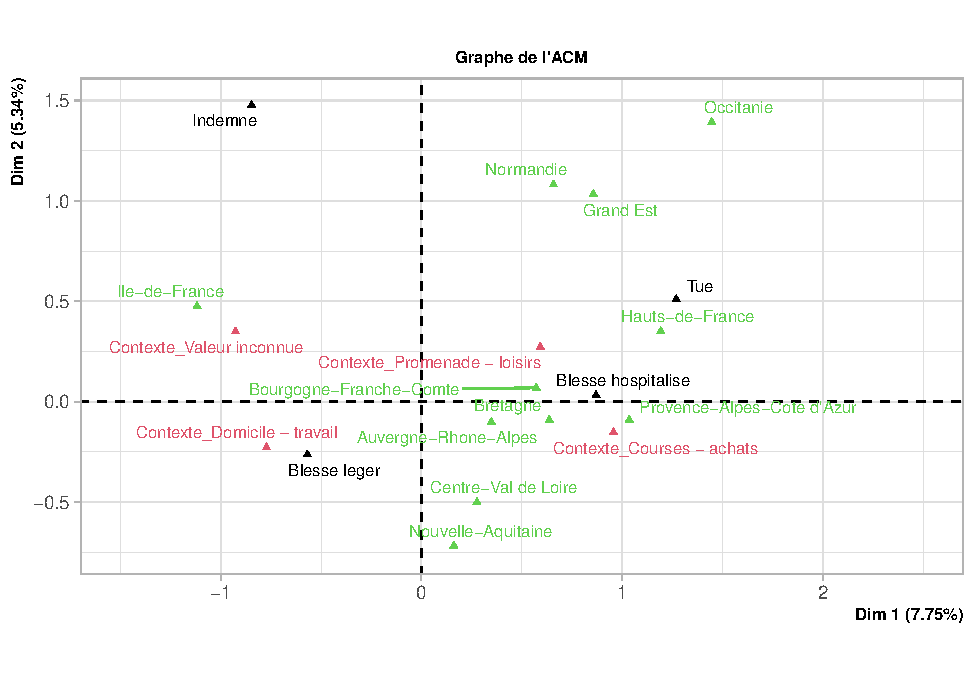
\includegraphics[width=0.9\linewidth]{Rapport_ADD_LEO-GABET_files/figure-latex/acm1modaCONTEXTE-1} 

}

\caption{AVEC CONTEXTE}\label{fig:acm1modaCONTEXTE}
\end{figure}

Le contexte domicile-travail est mise en avant pour le cas des blessé léger qui est fortement influencé par la région Ile de France. Tout court, cette région influence totalement toute la partie Gauche de notre graphe.
Tant dis que le coté droit du graphe, on retrouve logiquement les cas plus grave en accient dont le contexte Courses-achats et Promenade-loisirs qui est mise en avant.
Ceci nous permet d'analyser que les cas d'accident les plus graves se produisent lors des moments de détentes, donc renforcer les préventions en mettant en avant les chiffres d'accident de vélo dans le contexte de loisir pourrait sensibiliser davantage la population.

\hypertarget{afc-sur-les-ruxe9gions-selon-les-consuxe9quences}{%
\subsubsection{AFC sur les régions selon les conséquences}\label{afc-sur-les-ruxe9gions-selon-les-consuxe9quences}}

\begin{verbatim}
##                             V2
## V1                           Blesse hospitalise Blesse leger Indemne  Tue
##   Auvergne-Rhone-Alpes                      561          567      75   85
##   Bourgogne-Franche-Comte                   192          153      22   26
##   Bretagne                                  414          347      34   54
##   Centre-Val de Loire                       256          301      39   21
##   Corse                                      20           10       3    4
##   Grand Est                                 391          271      48   39
##   Hauts-de-France                           184           78       8   23
##   Ile-de-France                             386         2156     367   22
##   Normandie                                 106          135      16   21
##   Nouvelle-Aquitaine                        529          684      63   62
##   Occitanie                                 109           43       6   14
##   Pays de la Loire                          413          659      61   52
##   Provence-Alpes-Cote d'Azur                 90           57       1   14
\end{verbatim}

\begin{verbatim}
## 
##  Pearson's Chi-squared test
## 
## data:  contingence
## X-squared = 1430.8, df = 36, p-value < 2.2e-16
\end{verbatim}

\begin{figure}[H]

{\centering 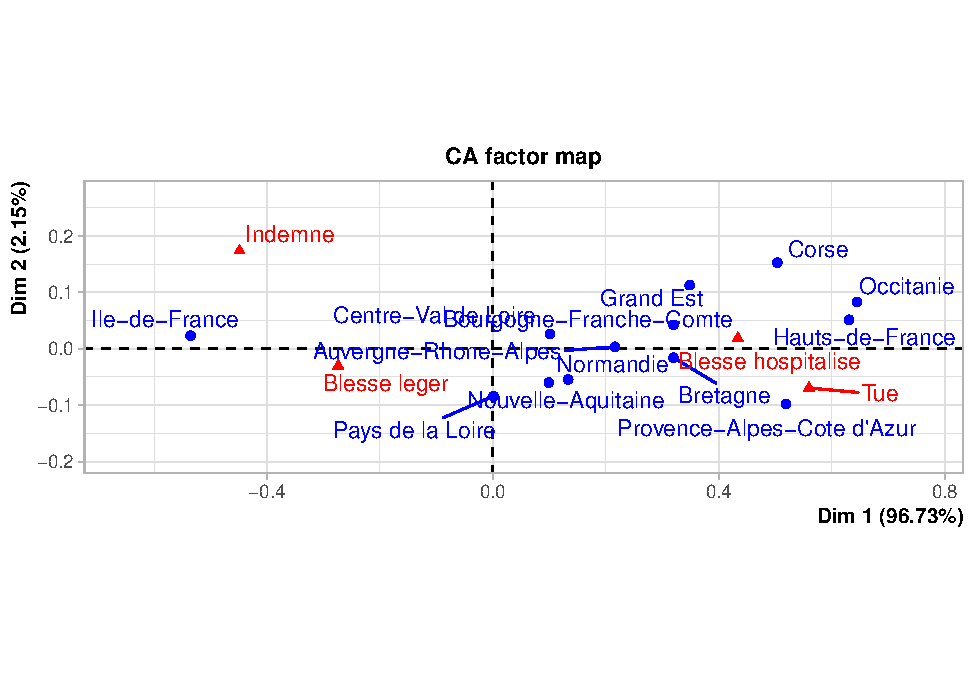
\includegraphics[width=0.9\linewidth]{Rapport_ADD_LEO-GABET_files/figure-latex/afc1-1} 

}

\caption{AFC1}\label{fig:afc1}
\end{figure}

Le test du chi carré indique une dépendance significative entre les variables, avec un p-value très faible (1.988227e-277). Cela suggère que les caractéristiques analysées ne sont pas indépendantes.

Les valeurs propres représentent la variance expliquée par chaque dimension. La première dimension explique 96.728\% de la variance, la deuxième 2.150\%, et la troisième 1.122\%. La première dimension est donc prédominante.

Les résultats pour les départements montrent leurs positions sur les dimensions extraites. Par exemple, l'Ile-de-France est fortement associée à la première dimension (Dim.1), mais négativement.

Les résultats pour les conséquences des accidents montrent leur association avec les dimensions extraites. Par exemple, ``Blesse hospitalise'' est positivement associé à la première dimension, tandis que ``Indemne'' est négativement associé.

\begin{figure}[H]

{\centering 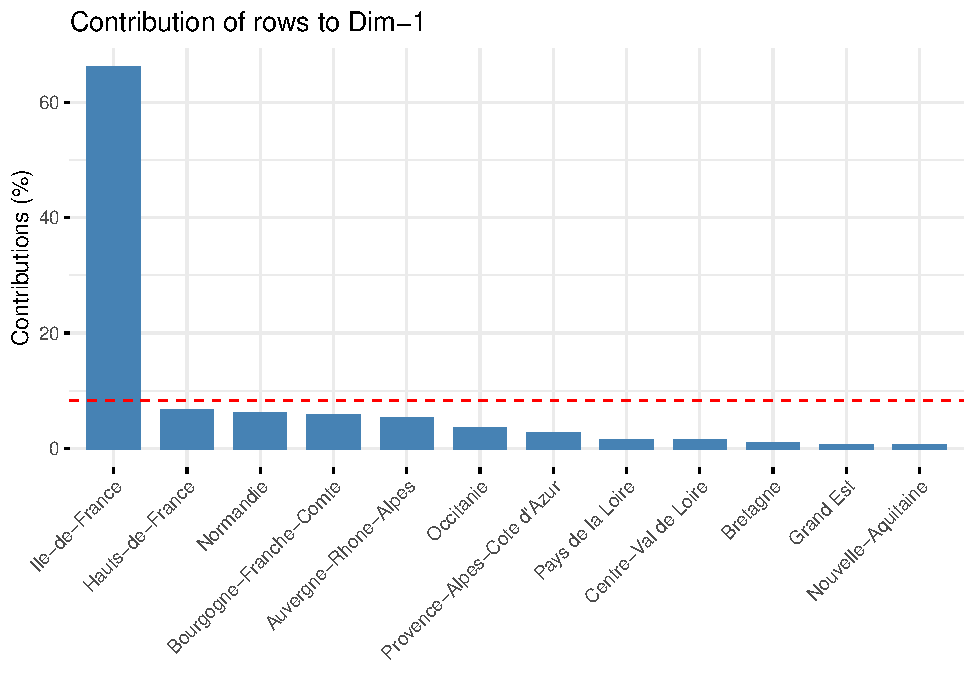
\includegraphics[width=0.9\linewidth]{Rapport_ADD_LEO-GABET_files/figure-latex/afc2-1} 

}

\caption{AFC2}\label{fig:afc2}
\end{figure}

\begin{figure}[H]

{\centering 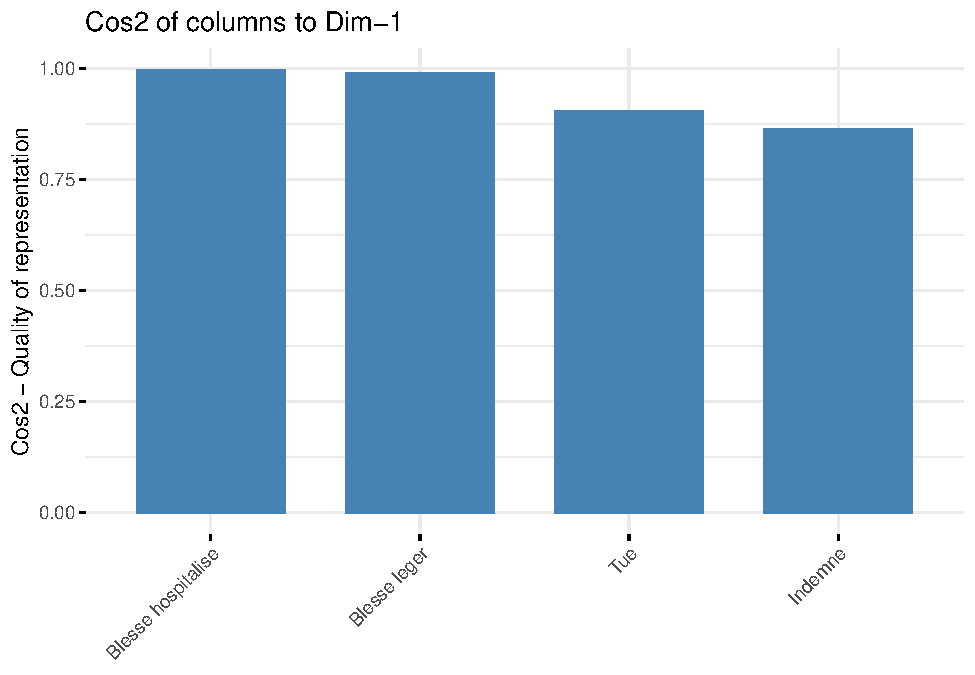
\includegraphics[width=0.9\linewidth]{Rapport_ADD_LEO-GABET_files/figure-latex/afc3-1} 

}

\caption{AFC3}\label{fig:afc3}
\end{figure}

Les valeurs \(cos^2\) proches de 1 indiquent une bonne représentation. Par exemple, ``Blesse hospitalise'' à un \(cos^2\) élevé sur la première dimension.

Interprétation Générale :

\begin{itemize}
\item
  La première dimension semble être associée à des caractéristiques qui différencient les départements, peut-être liées à la prévalence des accidents. L'Ile-de-France se distingue par une contribution de 60\%, ce qui pourrait indiquer des facteurs spécifiques à cette région (que nous verrons par la suite).
\item
  La conséquence ``Tué'' est associée à la première dimension, ce qui indique que sa fréquence est liée à des caractéristiques spécifiques des départements.
\item
  Le \(cos^2\) élevé pour ``Tué'' sur la troisième dimension suggère une spécificité dans les caractéristiques associées aux décès.
\end{itemize}

Donc, l'AFC met en évidence des associations significatives entre les départements, les conséquences des accidents, et les dimensions extraites. L'Ile-de-France se démarque et des patterns spécifiques méritent une exploration plus approfondie pour comprendre les facteurs qui contribuent aux accidents de vélo dans la région.

\hypertarget{acm-sur-la-muxe9tropole}{%
\subsection{ACM sur la métropole}\label{acm-sur-la-muxe9tropole}}

A partir de maintenant, nous allons étudié plus en détail la ville de Paris qui représente la majorité des cas d'accident de vélo en Ile de France.

\begin{figure}[H]

{\centering 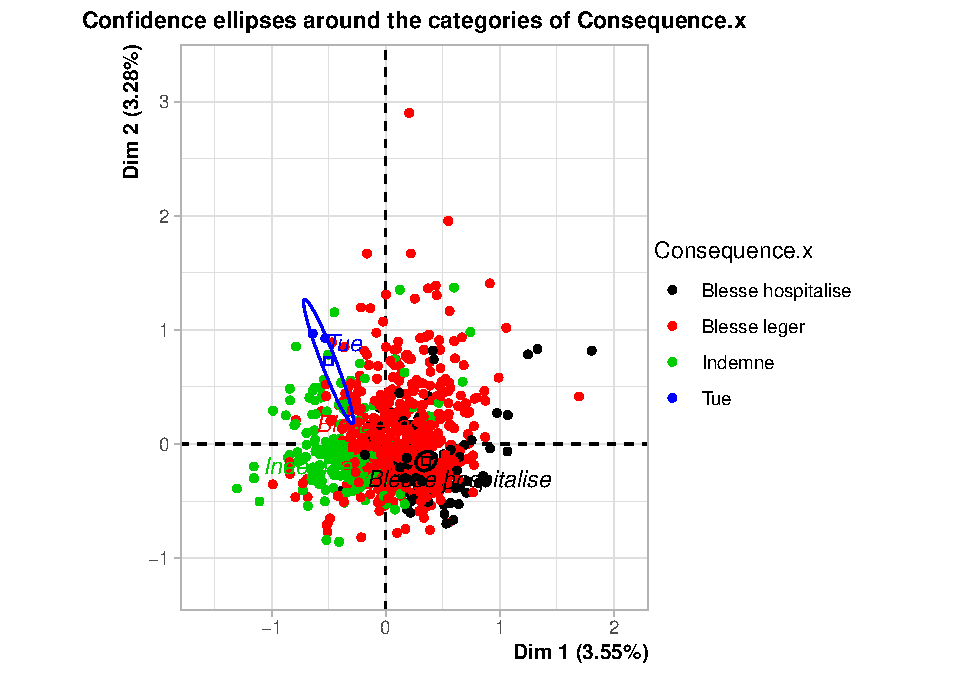
\includegraphics[width=0.9\linewidth]{Rapport_ADD_LEO-GABET_files/figure-latex/acmPARIS1-1} 

}

\caption{ACM PARIS}\label{fig:acmPARIS1}
\end{figure}

On retrouve une grande part d'accident léger parmis nos individus sur la partie gauche de notre graphe, consitué des quelques cas d'accidents plus graves.

Regardons de plus prêt nos variables associés :

\begin{figure}[H]

{\centering 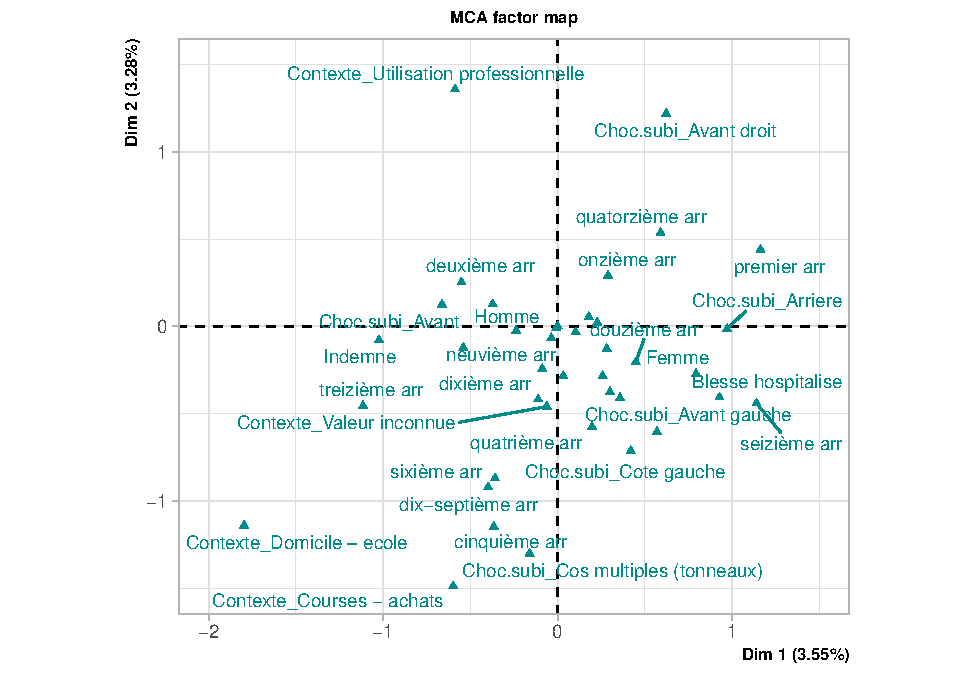
\includegraphics[width=0.9\linewidth]{Rapport_ADD_LEO-GABET_files/figure-latex/acmPARIS-1} 

}

\caption{ACM PARIS avec var}\label{fig:acmPARIS}
\end{figure}

Le mois de juin se démarque très particulièrement dans l'ensemble de la majorité des accidents, avec un très grand nombre de choc subi par le coté droit. De plus le contexte de loisir promenade est de nouveau présent, tout comme lors de notre analyse à l'échelle nationale.

\begin{verbatim}
##                   V2
## V1                 Blesse hospitalise Blesse leger Indemne Tue
##   cinquième arr                     1           23       5   0
##   deuxième arr                      9          109      37   0
##   dix-huitième arr                  4           57      14   0
##   dix-neuvième arr                 10           65      25   0
##   dix-septième arr                  2           29       7   0
##   dixième arr                       4           78      18   0
##   douzième arr                      7           67       8   0
##   huitième arr                      1           15       2   0
##   neuvième arr                      0           17       4   0
##   onzième arr                       2           52       9   0
##   premier arr                       9           35       5   0
##   quatorzième arr                   3           52      10   0
##   quatrième arr                    10           53      24   0
##   quinzième arr                     4           50       9   2
##   seizième arr                      2           14       0   0
##   septième arr                      5           46       7   0
##   sixième arr                       8           44      20   0
##   treizième arr                     2           38      18   0
##   troisième arr                    11           66      23   0
##   vingtième arr                     3           58       8   1
\end{verbatim}

\begin{verbatim}
## 
##  Pearson's Chi-squared test
## 
## data:  contingence
## X-squared = 95.305, df = 57, p-value = 0.001105
\end{verbatim}

\begin{figure}[H]

{\centering 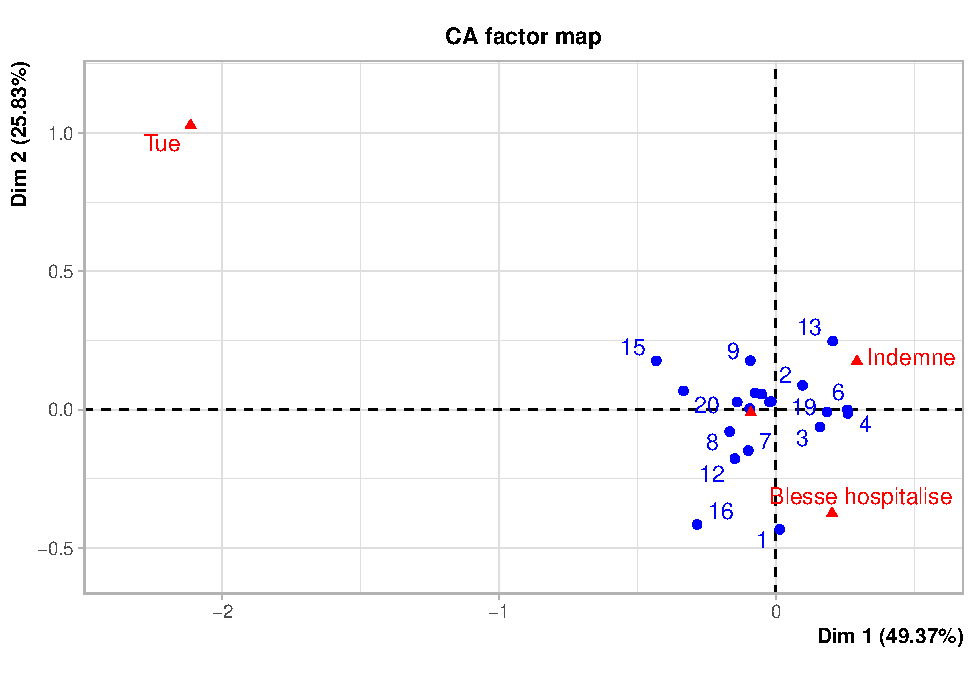
\includegraphics[width=0.9\linewidth]{Rapport_ADD_LEO-GABET_files/figure-latex/Afc2PARIS-1} 

}

\caption{AFC PARIS}\label{fig:Afc2PARIS}
\end{figure}

\begin{verbatim}
##                              V2
## V1                            Blesse hospitalise Blesse leger Indemne Tue
##   Courses - achats                             0            4       2   0
##   Domicile – ecole                             1           20       7   0
##   Domicile – travail                          20          245      58   0
##   Non renseigne                               27          244      61   2
##   Promenade - loisirs                         30          291      67   1
##   Utilisation professionnelle                  8          102      36   0
##   Valeur inconnue                             11           62      22   0
\end{verbatim}

\begin{verbatim}
## 
##  Pearson's Chi-squared test
## 
## data:  contingence
## X-squared = 15.208, df = 18, p-value = 0.6476
\end{verbatim}

\begin{figure}[H]

{\centering 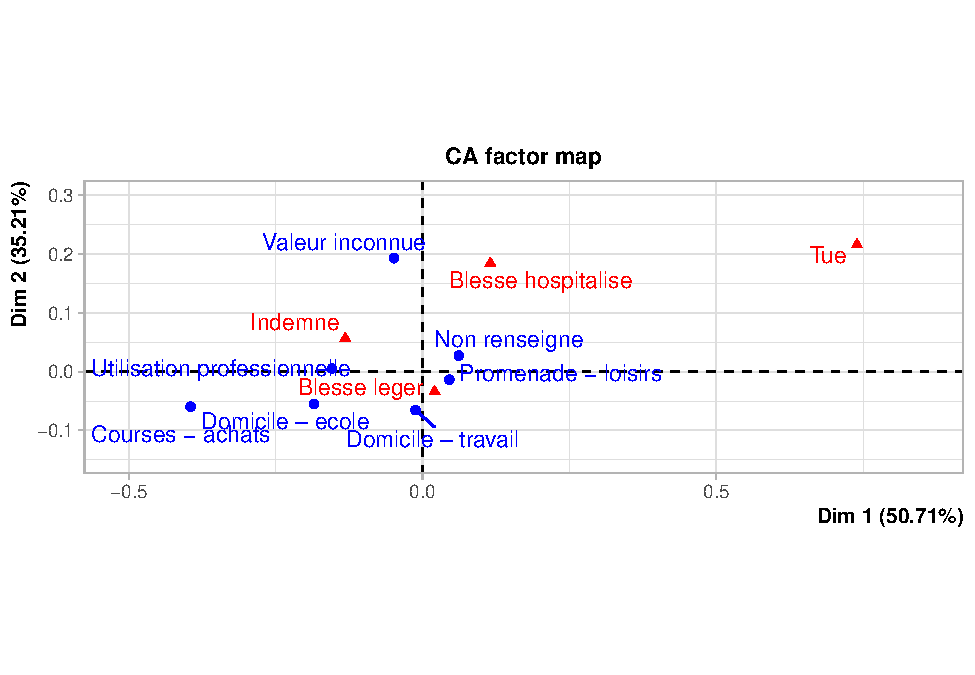
\includegraphics[width=0.9\linewidth]{Rapport_ADD_LEO-GABET_files/figure-latex/Afc3PARIS-1} 

}

\caption{AFC PARIS}\label{fig:Afc3PARIS}
\end{figure}

\hypertarget{afc-sur-les-pistes-cyclables-de-paris}{%
\subsection{AFC sur les pistes cyclables de Paris}\label{afc-sur-les-pistes-cyclables-de-paris}}

\begin{verbatim}
##     V2
## V1   Autres itineraires cyclables (ex : Aires pietonnes - Contre-sens cyclables)
##   1                                                                          139
##   10                                                                         108
##   11                                                                         250
##   12                                                                         216
##   13                                                                         260
##   14                                                                         217
##   15                                                                         311
##   16                                                                          92
##   17                                                                         194
##   18                                                                         369
##   19                                                                         172
##   2                                                                          144
##   20                                                                         312
##   3                                                                           94
##   4                                                                          198
##   5                                                                          232
##   6                                                                          158
##   7                                                                          159
##   8                                                                           28
##   9                                                                           98
##     V2
## V1   Bandes cyclables Couloirs de bus ouverts aux velos Pistes cyclables
##   1                25                               107               17
##   10              100                                73              235
##   11               62                                26              193
##   12              120                                96              627
##   13              153                               170              589
##   14              131                               145              343
##   15              156                                99              333
##   16              108                               107              314
##   17              340                               116              200
##   18               88                               124              270
##   19              110                                78              353
##   2                47                                46               10
##   20              129                                41              341
##   3                13                                62               16
##   4                62                                75              225
##   5               102                                64               69
##   6                81                                99               23
##   7                76                                60               58
##   8               152                               128              267
##   9                76                               135               37
\end{verbatim}

\begin{figure}[H]

{\centering 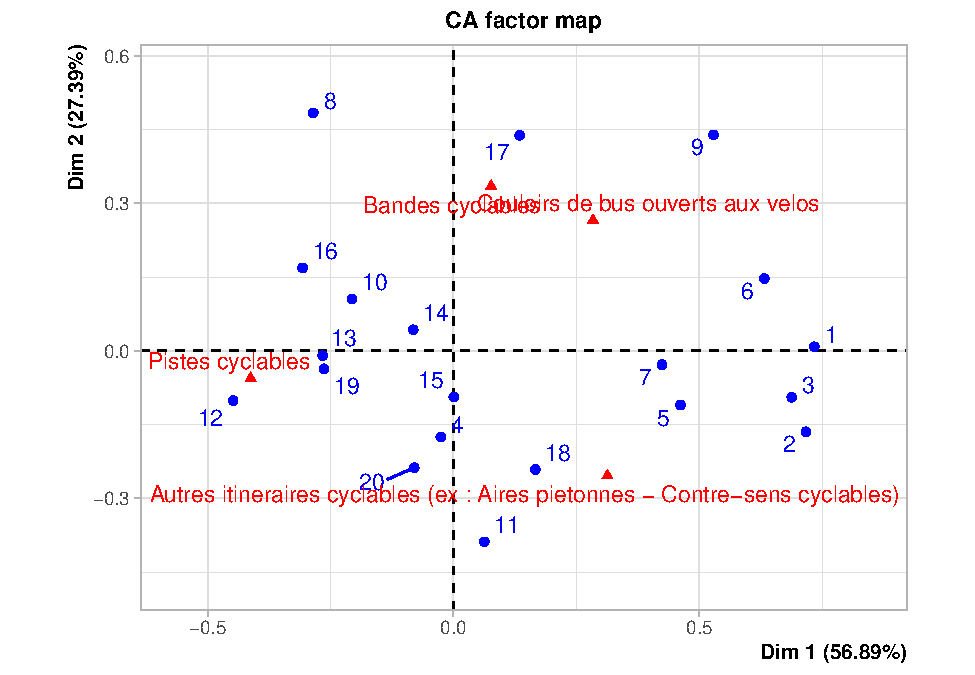
\includegraphics[width=0.9\linewidth]{Rapport_ADD_LEO-GABET_files/figure-latex/Afc5PARISvelo-1} 

}

\caption{AFC PARIS pistes}\label{fig:Afc5PARISvelo}
\end{figure}




\end{document}
